\chapter{模板的使用方法}
该模板适用于texlive2020系统,用以排版中南大学学位论文。
\section{公式的排版}
定理:$\sin^2\theta + \cos^2\theta = 1$。(行内公式不带编号)
\begin{equation}
\lim\limits_{xy\to 10}\frac{\sin xy}{xy} = 1
\end{equation}
\begin{equation}
\sum_{x=0}^{n}x^2 \quad \int_{x=0}^{n}x^2 \mathrm{d}x
\end{equation}
\begin{eqnarray} 
\dot{x}(t)=\bar{A}_{i}x(t)+\bar{B}_{i_{1}}x(t)+\bar{B}_{i_{2}}x(t)+\bar{B}_{i_{3}}[a_{i}(t)+b_{i}(t)].
\end{eqnarray}

\section{算法的排版}
基于。。。。原理,我们设计了高效的的算法来求解该问题,如\algref{alg:a}所示。
\begin{algorithm} 
	\caption{Identify Row Context} \label{alg:a}
	\KwIn{$r_i$, $Backgrd(T_i)$=${T_1,T_2,\ldots ,T_n}$ and similarity threshold $\theta_r$} 
	\KwOut{$con(r_i)$} 
	$con(r_i)= \Phi$\; 
	\For{$j=1;j \le n;j \ne i$}{ 
		float $maxSim=0$\; 
		$r^{maxSim}=null$\; 
		\While{not end of $T_j$}{ 
			compute Jaro($r_i,r_m$)($r_m\in T_j$)\; 
			\If{$(Jaro(r_i,r_m) \ge \theta_r)\wedge (Jaro(r_i,r_m)\ge r^{maxSim})$}{ 
				replace $r^{maxSim}$ with $r_m$\; 
			} 
		} 
		$con(r_i)=con(r_i)\cup {r^{maxSim}}$\; 
	} 
	\Return $con(r_i)$\; 
\end{algorithm}

\section{表格的排版}

\subsection{普通表格}
\tblref{tab:commontable} 是一个普普通通的表格。
\begin{table}[h]
	\centering % centering table
	\caption{这是一个普普通通的表格}
	\begin{tabular}{lccc}
		\toprule
		Package&Text&Greek&CM sym\\
		\midrule
		computer modern&cm&cm&ss\\
		cmbright&cmbright&cmbright&cm*\\
		ccfonts,eulervm&concrete&euler&euler\\
		concmath&concrete&concrete&concmath\\
		iwona&iwona&iwona&iwona\\
		kurier&kurier&kurier&kurier\\
		anttor&anttor&anttor&anttor\\
		kmath,kerkis&kerkis&kerkis&txfonts\\
		millennial&nc schlbk&millennial&txfonts\\
		\bottomrule
	\end{tabular}
	\label{tab:commontable}
\end{table}

\subsection{这是一个带脚注的表格}
\tblref{tbl:notetable} 是一个带脚注的表格。
\begin{table*}[!h]
	\scriptsize
	\centerfloat
	\caption{这是一个带脚注的表格}\label{tbl:notetable}
	\begin{threeparttable}
		\begin{tabular}{lcrrrrrrrrrrrrrrrr}
			\toprule
			\multirow{2}{*}{Inst.}&\multirow{2}{*}{$m$}&\multirow{2}{*}{$n$}&\multicolumn{3}{c}{GUROBI}&\multicolumn{4}{c}{Zhang's VNS}&\multicolumn{4}{c}{Qiu's TS}&\multicolumn{4}{c}{proposed ATS}\\
			\cmidrule(r){4-6}\cmidrule(r){7-10}\cmidrule(r){11-14}\cmidrule(r){15-18}
			&&&$opt./UB$&$gap\%$&$CPU$(s)&$gap\%$&std&$|K|$&$CPU$(s)&$gap\%$&std&$|K|$&$CPU$(s)&$gap\%$&std&$|K|$&$CPU$(s)\\
			
			\midrule
			2\_5&2&5&75.59 &0.00&0.17 &0.00&0.00 &1.0 &5.35 &0.00&0.00 &1.0 &1.46 &0.00&0.00 &1.0 &2.40 \\
			2\_6&2&6&68.40 &0.00&0.17 &0.00&0.00 &1.0 &5.75 &0.00&0.00 &1.0 &1.71 &0.00&0.00 &1.0 &2.60 \\
			2\_7&2&7&123.97 &0.00&0.32 &1.23&0.16 &2.0 &11.99 &\textbf{0.76}&0.81 &2.0 &2.55 &1.27&0.00 &2.0 &4.06 \\
			2\_8&2&8&78.44 &0.00&0.19 &0.00&0.00 &1.0 &5.61 &0.00&0.00 &1.0 &1.97 &0.00&0.00 &1.0 &3.09 \\
			2\_9&2&9&76.98 &0.00&0.56 &0.00&0.00 &1.0 &6.22 &0.00&0.00 &1.0 &2.10 &0.00&0.00 &1.0 &3.36 \\
			2\_10&2&10&89.03 &0.00&20.82 &0.45&0.24 &1.0 &5.41 &8.48&14.18 &1.1 &2.12 &\textbf{0.00}&0.00 &1.0 &3.51 \\
			2\_11&2&11&88.77 &0.00&52.59 &0.85&0.17 &1.0 &5.59 &16.63&20.68 &1.3 &2.54 &\textbf{0.74}&0.00 &1.0 &3.64 \\
			3\_5&3&5&70.75 &0.00&0.33 &0.00&0.00 &1.0 &5.36 &0.00&0.00 &1.0 &1.46 &0.00&0.00 &1.0 &2.37 \\
			3\_6&3&6&131.69 &0.00&1.22 &0.00&0.00 &2.0 &18.28 &0.00&0.00 &2.0 &2.27 &0.00&0.00 &2.0 &4.51 \\
			3\_7&3&7&75.16 &0.00&1.27 &0.00&0.00 &1.0 &6.36 &0.00&0.00 &1.0 &1.77 &0.00&0.00 &1.0 &2.89 \\
			3\_8&3&8&127.80 &0.00&3.00 &0.00&0.00 &2.0 &19.37 &0.00&0.00 &2.0 &2.69 &0.00&0.00 &2.0 &4.22 \\
			3\_9&3&9&126.76 &0.00&1.94 &0.43&0.00 &2.0 &34.93 &0.43&0.00 &2.0 &3.08 &0.43&0.00 &2.0 &4.73 \\
			3\_10&3&10&139.57 &0.00&27.52 &0.16&0.14 &2.0 &27.30 &0.16&0.18 &2.0 &2.99 &\textbf{0.00}&0.00 &2.0 &5.93 \\
			3\_11&3&11&128.05 &0.00&8.18 &1.23&1.03 &2.0 &35.68 &0.27&0.19 &2.0 &3.42 &\textbf{0.00}&0.00 &2.0 &6.69 \\
			3\_12&3&12&139.37 &0.00&195.38 &1.42&0.47 &2.0 &13.09 &0.68&0.82 &2.0 &4.25 &\textbf{0.00}&0.00 &2.0 &6.55 \\
			4\_19&4&19&196.39 &\underline{26.39} &7200.08 &-17.77&2.66 &2.0 &28.75 &-20.17&3.65 &2.0 &5.08 &\textbf{-23.12}&0.51 &2.0 &9.07 \\
			4\_20&4&20&196.16 &\underline{25.92} &7200.09 &-14.89&1.58 &2.0 &39.05 &-0.45&13.39 &2.9 &6.82 &\textbf{-21.83}&2.06 &2.0 &9.34 \\
			AVG&&&&&&2.62&&&&2.38&&&&\textbf{0.29}&&&\\
			\bottomrule
		\end{tabular}
		\begin{tablenotes}
			\footnotesize
            \item 注:
			\item (1) The \underline{underlined} $gap\%$ shows that the corresponding solutions have large gaps. The last two rows of \tblref{tbl:notetable} imply that the GUROBI can not obtain the corresponding optimal solutions. 
            \item (2) The values in \textbf{boldface} are the best known solutions among the above three heuristic algorithms. 
		\end{tablenotes}
	\end{threeparttable}
\end{table*}



\subsection{横向表格}
\tblref{tbl:landscapetable} 是一个横向表格。
\begin{landscape} 
	\begin{table}
		\caption{这是一个横向表格}\label{tbl:landscapetable}
		\begin{tabular}{lccccccc}
			\toprule
			Package&Text&Greek&CM sym&AMS sym&Calligr&Blkbd&boldmath\\
			\midrule
			computer modern&cm&cm&cm&ams&cm&ams&yes\\
			cmbright&cmbright&cmbright&cm*&cm*&cm*&ams&no\\
			ccfonts,eulervm&concrete&euler&euler&ams&euler&ams&yes\\
			concmath&concrete&concrete&concmath&concmath&concmath&concmath&no\\
			iwona&iwona&iwona&iwona&iwona&cm*&ams&yes\\
			kurier&kurier&kurier&kurier&kurier&cm*&ams&yes\\
			anttor&anttor&anttor&anttor&anttor&anttor&ams&yes\\
			kmath,kerkis&kerkis&kerkis&txfonts&txfonts&txfonts&txfonts&yes\\
			millennial&nc schlbk&millennial&txfonts&txfonts&txfonts&ams&no\\
			fouriernc&nc schlbk&fourier&fourier&fourier&fourier&fourier&yes\\
			pxfonts&palatino&pxfonts&txfonts*&txfonts*&txfonts*&pxfonts&yes\\
			mathpazo&palatino&pazo&cm&ams&cm&pazo&yes\\
			mathpple&palatino&euler&euler&ams&cm&ams&yes\\
			txfonts&times&txfonts&txfonts&txfonts&txfonts&txfonts&yes\\
			mathtime (Belleek)&times&belleek&belleek&ams&cm&ams&no\\
			mathptmx&times&symbol&cm&ams&rsfs&ams&no\\
			mbtimes&omega&omega&mbtimes&ams&rsfs*&esstix&yes\\
			mathdesign (Charter)&charter&md charter&md charter&md charter& rsfs* &ams&yes\\
			arev&arev&arev&md charter&md charter&cm&fourier&yes\\
			mathdesign (Garamond)&garamond&md garamond&md garamond&md garamond& rsfs* & ams* &yes\\
			fourier&utopia&fourier&fourier&fourier&fourier&fourier&yes\\
			mathdesign (Utopia)&utopia&md garamond&md utopia&md utopia&rsfs*&ams*&yes\\
			\bottomrule
		\end{tabular}
	\end{table}
\end{landscape} 


\subsection{横向长表格}
\tblref{tbl:long-tabu} 是一个横向长表格
\begin{landscape} 
\begin{spacing}{1}
	
	\begin{longtable}{lccccccc}	
		\caption{这是一个横向长表格}\label{tbl:long-tabu}\\
		\toprule
		Package&Text&Greek&CM sym&AMS sym&Calligr&Blkbd&boldmath\\
		\midrule
		\endfirsthead
		\multicolumn{8}{l}{\kaishu 续\tblref{tbl:long-tabu}} \\
		\toprule
		Package&Text&Greek&CM sym&AMS sym&Calligr&Blkbd&boldmath\\
		\midrule
		\endhead
		\midrule 
		\multicolumn{8}{r}{\kaishu 接下页} \\
		\endfoot
		\bottomrule
		\endlastfoot
		computer modern&cm&cm&cm&ams&cm&ams&yes\\
		cmbright&cmbright&cmbright&cm*&cm*&cm*&ams&no\\
		ccfonts,eulervm&concrete&euler&euler&ams&euler&ams&yes\\
		concmath&concrete&concrete&concmath&concmath&concmath&concmath&no\\
		iwona&iwona&iwona&iwona&iwona&cm*&ams&yes\\
		kurier&kurier&kurier&kurier&kurier&cm*&ams&yes\\
		anttor&anttor&anttor&anttor&anttor&anttor&ams&yes\\
		kmath,kerkis&kerkis&kerkis&txfonts&txfonts&txfonts&txfonts&yes\\
		millennial&nc schlbk&millennial&txfonts&txfonts&txfonts&ams&no\\
		fouriernc&nc schlbk&fourier&fourier&fourier&fourier&fourier&yes\\
		pxfonts&palatino&pxfonts&txfonts*&txfonts*&txfonts*&pxfonts&yes\\
		mathpazo&palatino&pazo&cm&ams&cm&pazo&yes\\
		mathpple&palatino&euler&euler&ams&cm&ams&yes\\
		txfonts&times&txfonts&txfonts&txfonts&txfonts&txfonts&yes\\
		mathtime (Belleek)&times&belleek&belleek&ams&cm&ams&no\\
		mathptmx&times&symbol&cm&ams&rsfs&ams&no\\
		mbtimes&omega&omega&mbtimes&ams&rsfs*&esstix&yes\\
		mathdesign (Charter)&charter&md charter&md charter&md charter& rsfs* &ams&yes\\
		arev&arev&arev&md charter&md charter&cm&fourier&yes\\
		mathdesign (Garamond)&garamond&md garamond&md garamond&md garamond& rsfs* & ams* &yes\\
		fourier&utopia&fourier&fourier&fourier&fourier&fourier&yes\\
		mathdesign (Utopia)&utopia&md garamond&md utopia&md utopia&rsfs*&ams*&yes\\
		computer modern&cm&cm&cm&ams&cm&ams&yes\\
		cmbright&cmbright&cmbright&cm*&cm*&cm*&ams&no\\
		ccfonts,eulervm&concrete&euler&euler&ams&euler&ams&yes\\
		concmath&concrete&concrete&concmath&concmath&concmath&concmath&no\\
		iwona&iwona&iwona&iwona&iwona&cm*&ams&yes\\
		kurier&kurier&kurier&kurier&kurier&cm*&ams&yes\\
		anttor&anttor&anttor&anttor&anttor&anttor&ams&yes\\
		kmath,kerkis&kerkis&kerkis&txfonts&txfonts&txfonts&txfonts&yes\\
		millennial&nc schlbk&millennial&txfonts&txfonts&txfonts&ams&no\\
		fouriernc&nc schlbk&fourier&fourier&fourier&fourier&fourier&yes\\
		pxfonts&palatino&pxfonts&txfonts*&txfonts*&txfonts*&pxfonts&yes\\
		mathpazo&palatino&pazo&cm&ams&cm&pazo&yes\\
		mathpple&palatino&euler&euler&ams&cm&ams&yes\\
		txfonts&times&txfonts&txfonts&txfonts&txfonts&txfonts&yes\\
		mathtime (Belleek)&times&belleek&belleek&ams&cm&ams&no\\
		mathptmx&times&symbol&cm&ams&rsfs&ams&no\\
		mbtimes&omega&omega&mbtimes&ams&rsfs*&esstix&yes\\
		mathdesign (Charter)&charter&md charter&md charter&md charter& rsfs* &ams&yes\\
		arev&arev&arev&md charter&md charter&cm&fourier&yes\\
		mathdesign (Garamond)&garamond&md garamond&md garamond&md garamond& rsfs* & ams* &yes\\
		fourier&utopia&fourier&fourier&fourier&fourier&fourier&yes\\
		mathdesign (Utopia)&utopia&md garamond&md utopia&md utopia&rsfs*&ams*&yes\\
	\end{longtable}
\end{spacing}
\end{landscape}

\section{代码}
\begin{spacing}{1}
\begin{minted}{c++}
#include<iostream>
int main {
    std::cout<<"hello world"<<std::endl;
    std::cout<<"hello world"<<std::endl;
    std::cout<<"hello world"<<std::endl;
    std::cout<<"hello world"<<std::endl;
}
\end{minted}
\end{spacing}

\section{图片}
\subsection{普通图片}
\figref{fig:figure}是一张普普通通的图片。
\begin{figure}[htbp]
	\centering
	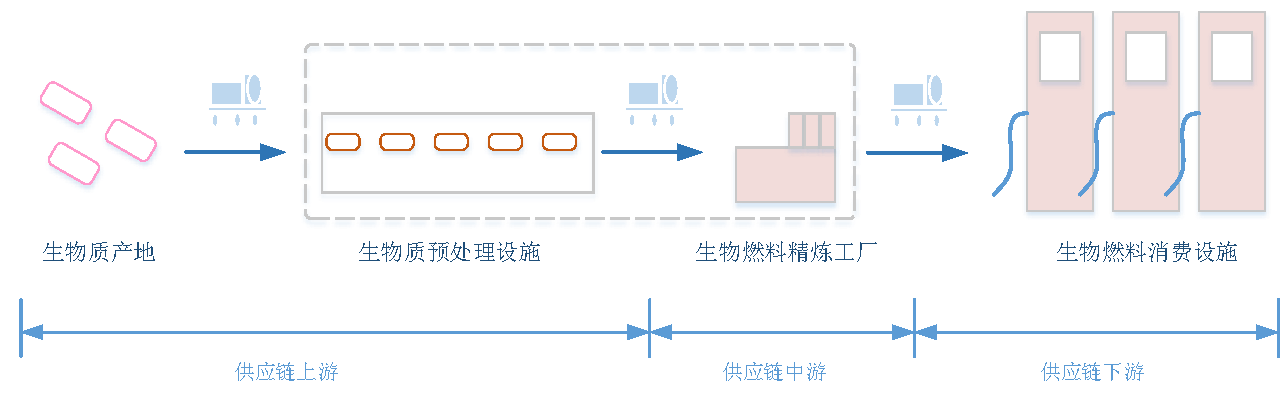
\includegraphics[width=\linewidth]{biofuelsc.pdf}
	\caption{生物燃料供应链示意图}
	\label{fig:figure}
\end{figure}

\subsection{子图}
\figref{fig:subfig}是母图,\figref{fig:subfig-A}和\figref{fig:subfig-B}是子图。
\begin{figure*}[ht]
	\centering
	\subfigure[子图A]{
		\label{fig:subfig-A}
		
\includegraphics[width=0.3\linewidth]{/csu/logo-blue}
	}
	\subfigure[子图B]{
		\label{fig:subfig-B}
		
\includegraphics[width=0.3\linewidth]{/csu/logo-orange}
	}
	\caption{这是子图的实例}
	\label{fig:subfig}
\end{figure*}

\subsection{横向图形}
\figref{fig:landscapefig} 是一个横向图片。
\begin{landscape}
	\begin{figure}
		\centering
		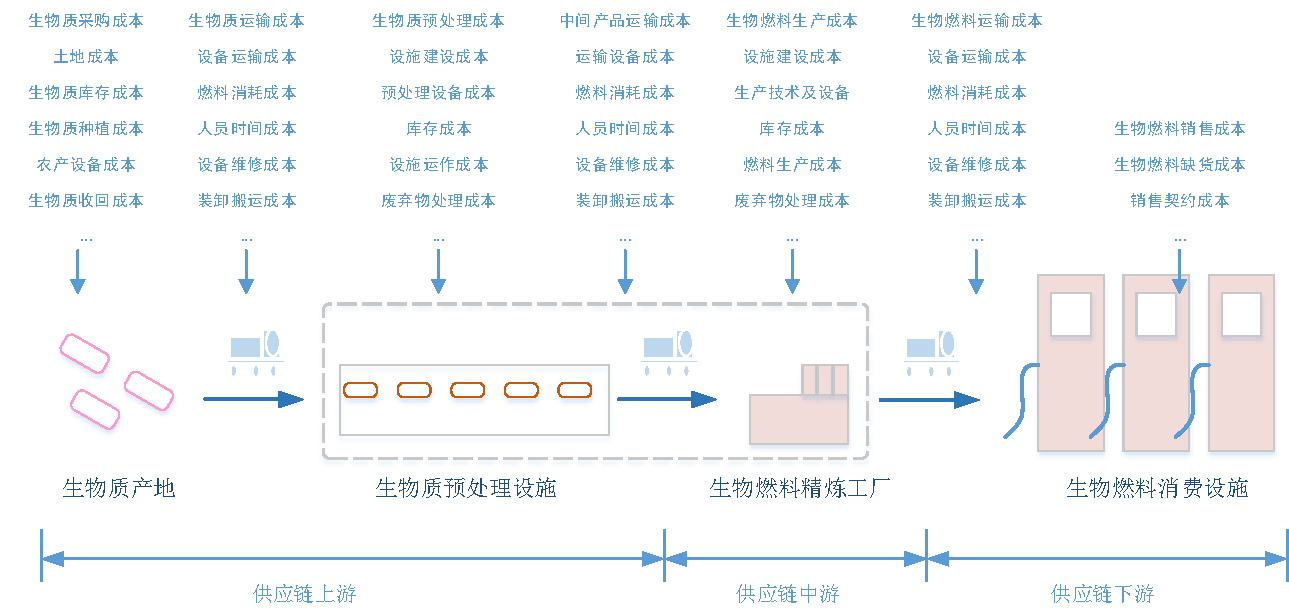
\includegraphics{biofuelcost.pdf}
		\caption{这是一个横向图片的实例}
		\label{fig:landscapefig}
	\end{figure}
\end{landscape}

\cleardoublepage